\documentclass[a4paper,12pt,abstracton]{scrartcl}
\usepackage[utf8]{inputenc}
\usepackage{float}
\usepackage{tikz}
\usepackage{amsmath}
\usepackage{amssymb}
\usepackage{pifont}% http://ctan.org/pkg/pifont
\usepackage[font=small,labelfont=bf]{caption}
\usepackage{graphicx}
%\usepackage{dirtytalk}
\usepackage{multicol}
\usepackage{booktabs}
\usepackage{colortbl}
\usepackage{appendix}
\usepackage{nomencl}
\usepackage{lmodern}
\usepackage[nottoc]{tocbibind}
\usepackage{xcolor}
%\graphicspath{images/}
\usepackage[margin = 3cm]{geometry}
\usepackage{ragged2e} % good alignment
\usepackage{hyperref}
\usepackage{siunitx} % Provides the \SI{}{} and \si{} command for typesetting SI units
\hypersetup{colorlinks=true,
    linkcolor=blue,
    filecolor=magenta,      
    urlcolor=cyan, 
    citecolor=gray}

%\DeclareGraphicsExtensions{.png,.pdf} % low-res (work in progress)
%\DeclareGraphicsExtensions{.pdf,.png}  % high-res (final draft)
%\setlength\parindent{0pt} % Removes all indentation from paragraphs
%\bibliographystyle{unstr}
\setlength\parindent{0pt}
\setlength{\parskip}{0.3em}
\newcommand{\xmark}{\ding{55}}

\renewcommand{\nomname}{List of Symbols}
\renewcommand{\nompreamble}{The following list explains the symbols used within the body of the report.}

\usepackage{etoolbox}
\renewcommand\nomgroup[1]{%
  \item[\bfseries
  \ifstrequal{#1}{E}{Experimental Equipment}{%
  \ifstrequal{#1}{C}{Computational Methods}{%
  \ifstrequal{#1}{T}{Theoretical Concepts}{
  \ifstrequal{#1}{P}{Physical Constants}{}}}}%
]}


\subject{CMP Lab Report} % Matter Physics, Physics, Chemical Physics ?
\title{Zeeman Effect}
\author{Group B9\footnote{Pietro Monticone , Claudio Moroni , Alberto Mosso , Riccardo Valperga.}}

\renewcommand{\listfigurename}{Plots}
\renewcommand{\listtablename}{Tables}
\renewcommand{\nomname}{Nomenclature}


\begin{document}
\maketitle
\makenomenclature
\tableofcontents
\newpage
\section{Anomlaous transverse Zeemann Effect}
Measures obtained:\newline
*****inserire tabelle*****
\begin{figure}[H]
\centering
\hspace*{-1.5cm}    
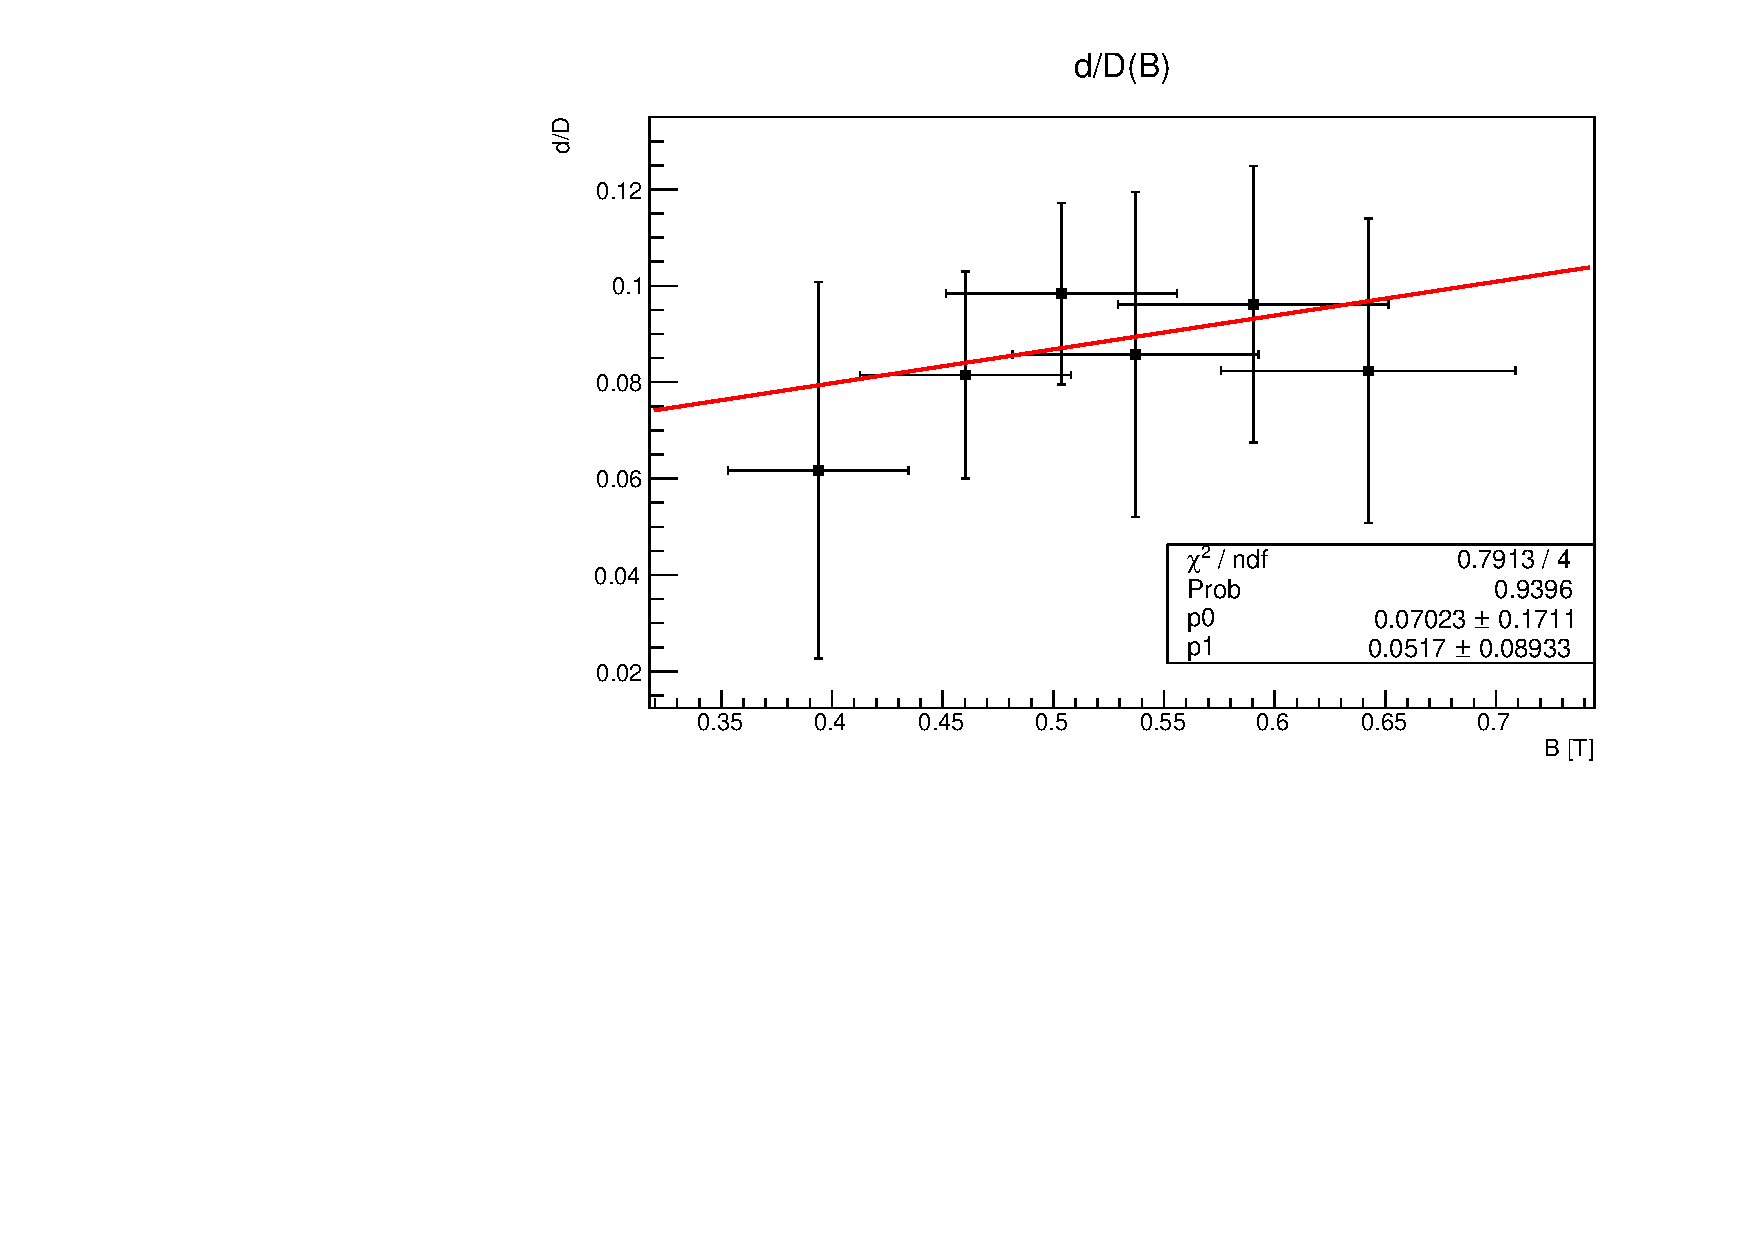
\includegraphics[trim=0cm 0cm 1.5cm 0cm,clip,width=17cm,keepaspectratio]{zat.pdf}
\end{figure}
From which we retrieve a value of $\mu_B$ of
\begin{equation*}
\mu_B =(3.192 \pm 7.799 )\times 10^{-24} \frac{J}{T}
\end{equation*}
Because of high data fluctuations, which very well exceed a $2 \sigma \; (95\% )$  criterion, it could be resolved to hypothesize that the $\delta \text{ and } \Delta $ measurements follow a gaussian distribution, and reject those data that lie further than $2 \sigma$ from the mean value. By doing so, one gets\newline
\begin{table}[H]
\centering
\resizebox{\linewidth}{!}{
\begin{tabular}{cccccc}
\toprule
I & sI & B & sB & dDm & sdDm\\
\midrule
\rowcolor{gray!6}  5.750 & 0.040 & 0.394 & 0.003 & 0.061 & 0.002\\
6.740 & 0.020 & 0.460 & 0.002 & 0.081 & 0.005\\
\rowcolor{gray!6}  7.275 & 0.025 & 0.504 & 0.009 & 0.082 & 0.008\\
7.820 & 0.020 & 0.537 & 0.009 & 0.085 & 0.003\\
\rowcolor{gray!6}  8.795 & 0.095 & 0.590 & 0.011 & 0.105 & 0.005\\
\addlinespace
9.950 & 0.040 & 0.642 & 0.011 & 0.108 & 0.007\\
\bottomrule
\end{tabular}}
\end{table}
\begin{figure}[H]
\centering
\hspace*{-1.5cm}    
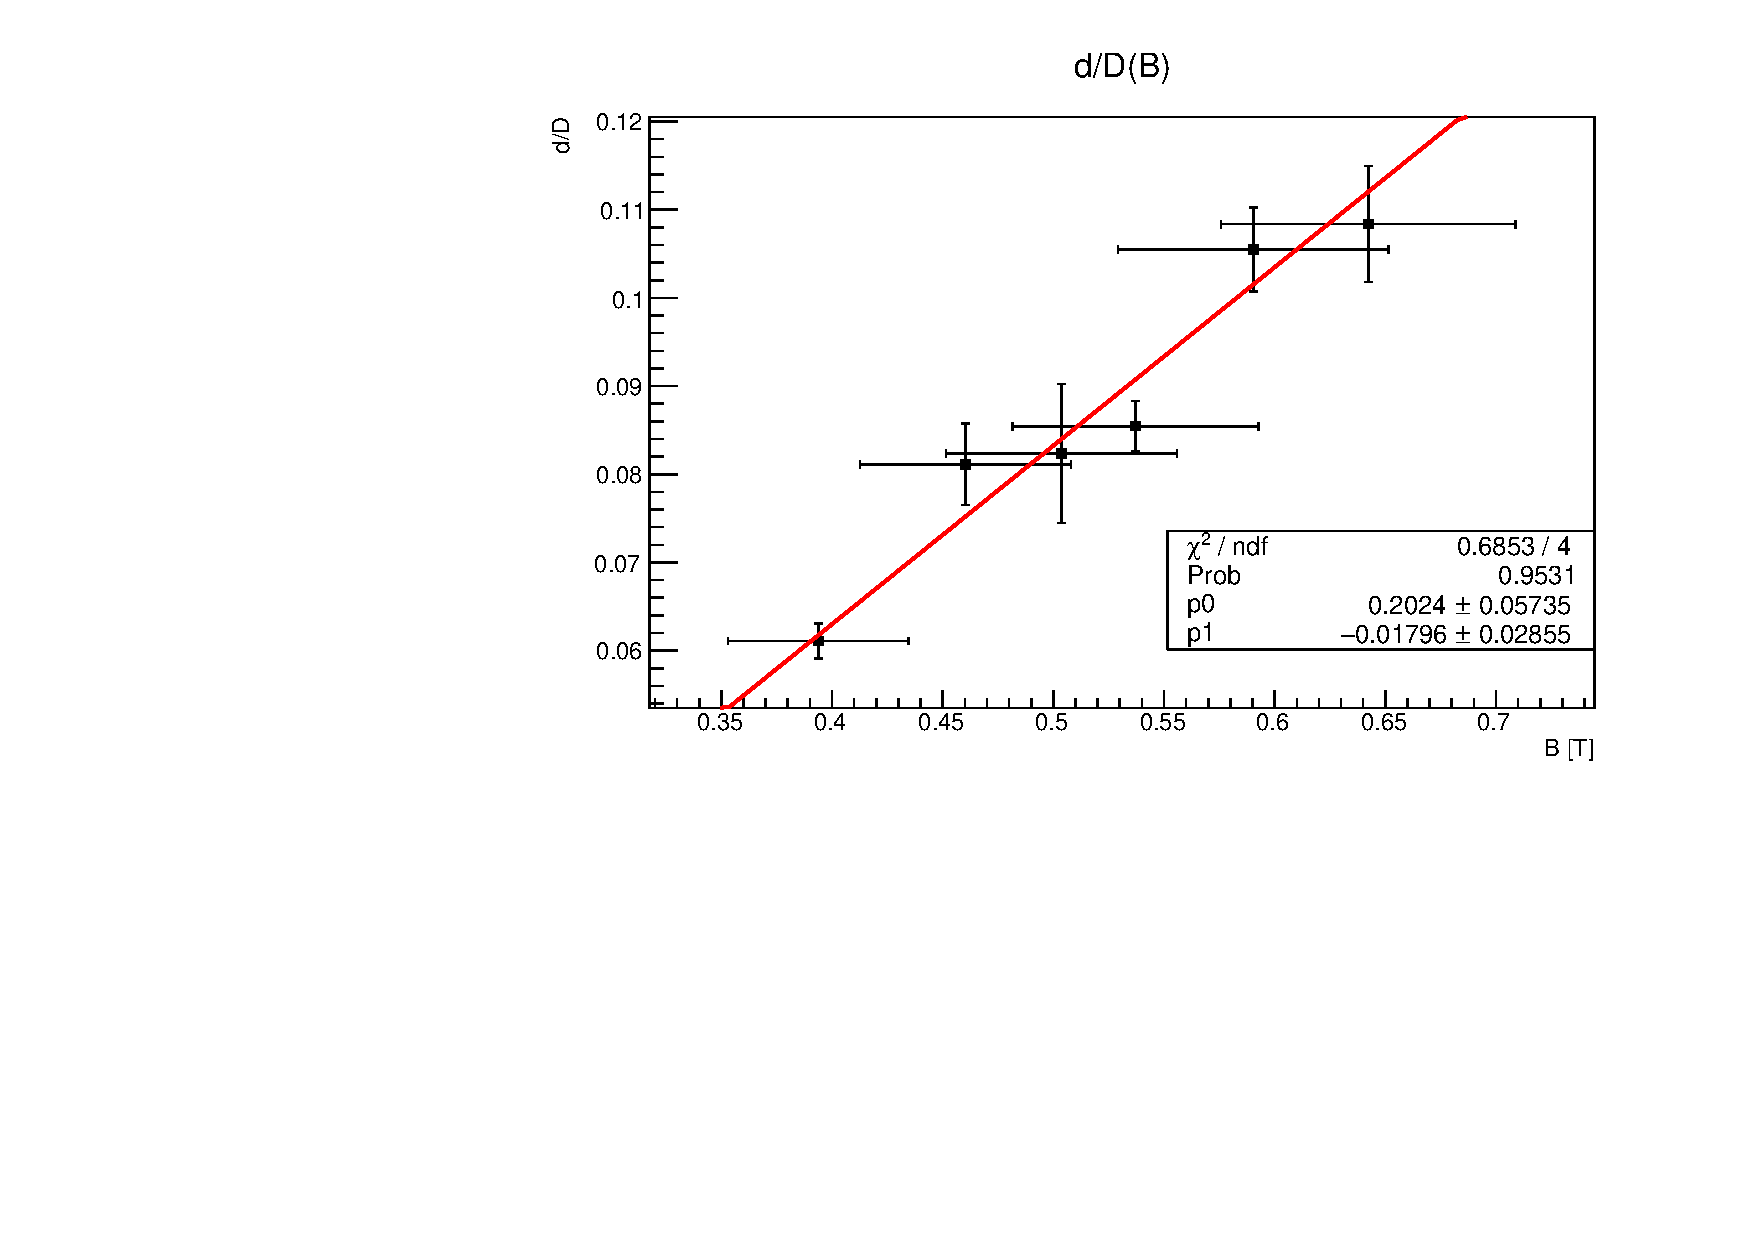
\includegraphics[trim=0cm 0cm 1.5cm 0cm,clip,width=17cm,keepaspectratio]{zatbs.pdf}
\end{figure}
Which gives 
\begin{equation*}
\mu_B =(9 \pm 2.599523 ) \times 10^{-24} \frac{J}{T}
\end{equation*}
That is the value we will use.

\end{document}
